\chapter{适应未知背景的可微分逆渲染方法}
\label{chap:method}

在重建3D人脸几何形状时,现有方法未能充分利用照片中的边缘信息。
它们大多依赖2D人脸关键点识别的结果来监督几何形状的优化,但这需要额外的标注步骤,且会引入累计误差,稀疏的关键点信息也会限制优化的精度。
也有方法利用传统的多目立体方法来确定几何形状,但这限制了其必须使用多视角照片作为输入。

很多3D人脸重建的现有方法也运用了可微分渲染技术,
这些方法都只针对每个像素的着色结果分别计算了梯度,但并没有考虑到由于模型间相互遮挡而导致的可见性梯度。
而该梯度正是所有梯度中的主要分量,对模型与照片中边缘的精确对齐有着重要作用。
另一方面,在通用的可微分渲染的相关研究中,
已经有很多方法可以高效地估计可见性梯度。
然而,计算正确的可见性梯度需要同时具有前景和背景的模型,但在非受限环境照片中,由于背景多样,很难得到准确的背景模型。

针对该问题,本章提出一种适应未知背景的可微分渲染方法,能够利用可见性梯度来优化模型,使其与照片中边缘精确对齐。
具体来说,本章提出了一种面积归一化的像素损失函数,通过收缩和扩展两项梯度详尽地说明了其性质,并介绍了一种高效实现的方式。
本章也通过实验证明了该损失函数确实能够使模型与照片中边缘精确对齐,同时无需背景模型,也不依赖关键点等额外监督信息。

\section{研究动机}

本章希望解决在利用可微分渲染的逆渲染优化过程中,3D人脸模型与照片中的边缘未能准确对齐的问题。
解决该问题的关键在于如何充分利用由于模型间相互遮挡而产生的可见性梯度。
现有基于可微分渲染的3D人脸重建方法都直接忽略了该项梯度。
而在通用可微分渲染的研究中,已经有很多方法可以高效地估计可见性梯度,但它们仍无法处理未知背景。
现有一个方法\citep{SchonbornEFV15}以概率推理的方式来重建人脸,它考虑了未知背景的情况,但其优化方式并非基于梯度,很难与其他方法结合。

\begin{figure}
\centering
\begin{tikzpicture}[
    every node/.style={draw, minimum size=1.3cm},
    data/.style={ellipse,fill=gray!20,minimum size=1.3cm},
    intermediate/.style={data,fill=none},
    param/.style={data,fill=blue!20},
    legend/.style={minimum size=0.5cm},
]
    \linespread{1.2}\small
    \node (render) {可微分渲染};
    \node (render_p) [below=of render,data] {渲染参数};
    \node [align=center] (model) [left=of render] {渲染参数\\预测模型};
    \node (model_p) [below=of model,param] {模型参数};
    \node (image) [right=of render,intermediate] {渲染图像};
    \node (loss) [right=of image, draw=red, thick] {损失函数};
    \node (photo) [below=of loss,data] {目标照片};

    \path [->] (render_p) edge (render)
               (model_p.100) edge (model_p.100|-model.south)
               (model.10) edge (model.10-|render.west)
               (image.170-|render.east) edge (image.170)
               (image.10) edge (image.10-|loss.west)
               (photo) edge (loss);
    \path [->, red, dashed] (image.350-|loss.west) edge (image.350)
                            (image.190) edge (image.190-|render.east)
                            (render.190) edge (render.190-|model.east)
                            (model.280) edge (model.280|-model_p.north);

    \node [right=1.5cm of loss, param, legend] (param_legend) {};
    \node [right=2pt of param_legend, draw=none] {可学习参数};

    \node [below=.2cm of param_legend, data, legend] (data_legend) {};
    \node [right=2pt of data_legend, draw=none] {固定数据};

    \node [below=.2cm of data_legend, legend, draw=none] (forward_legend) {};
    \path [->] ($(forward_legend) + (-.5, 0)$) edge ($(forward_legend) + (.3, 0)$);
    \node [right=2pt of forward_legend, draw=none] {前向传播};

    \node [below=.2cm of forward_legend, legend, draw=none] (backward_legend) {};
    \path [<-, red, dashed] ($(backward_legend) + (-.5, 0)$) edge ($(backward_legend) + (.3, 0)$);
    \node [right=2pt of backward_legend, draw=none] {反向传播};
\end{tikzpicture}
\caption{基于可微分渲染的逆渲染基本流程}
\label{fig:inv_rendering}
\end{figure}

本章方法是对可微分逆渲染流程的改进。
渲染指的是从渲染参数合成渲染图像的过程。
渲染参数的范围很广,以传统的基于3D网格的渲染为例,渲染参数可包括参数化的3D模型,如由三角形构成的3D网格的顶点坐标和其他属性,纹理贴图等,以及其他渲染参数,如相机参数,环境光照等。
而可微分渲染旨在计算渲染图像关于渲染参数的梯度。
该项技术通常应用于逆渲染的优化过程中,
如图\ref{fig:inv_rendering}是基于可微分渲染的逆渲染基本流程。
逆渲染过程通过计算渲染图像与目标照片之间的特定损失函数,并计算模型参数关于损失函数的梯度,以期利用基于梯度的方法优化输入参数,从而改善渲染效果,使之更加接近现实。
该思路在3D人脸重建的相关任务中已有较广泛的应用。
在3D人脸重建任务中,通常人脸3D模型是由另一个编码了人脸先验知识的模型预测而来,例如3DMM和/或神经网络。
基于梯度的优化方法也使得逆渲染方法可以方便地与神经网络结合,从而实现端到端的参数优化。

\subsection{通用可微分渲染无法处理未知背景}

然而现有通用可微分渲染方法仍无法处理未知背景:
现有方法对整张图片计算损失函数和估计梯度,即不区分前景和背景部分。
其中前景和背景间相互遮挡而产生的可见性梯度则需要渲染图像中同时包含较为准确的前景和背景才能得到。
但是,在基于非受限环境照片的人脸重建任务中,我们通常只有前景(即人脸)的3D模型,而没有背景的模型,因而无法渲染背景部分。
此时,现有方法选择忽略模型间相互遮挡产生的可见性梯度,而这会造成模型与照片的对齐不准确,如图\ref{fig:problem_a}所示。
另一方面,若对背景进行很粗糙的建模,例如假设为全黑,则错误的梯度会引导前景模型拟合背景,最终虽然能得到更低的损失函数,但模型的几何形状却不能收敛到期望的位置,如图\ref{fig:problem_b}所示。

\begin{figure}[p]
\centering
\begin{subfigure}[t]{0.5\textwidth}
    \centering
    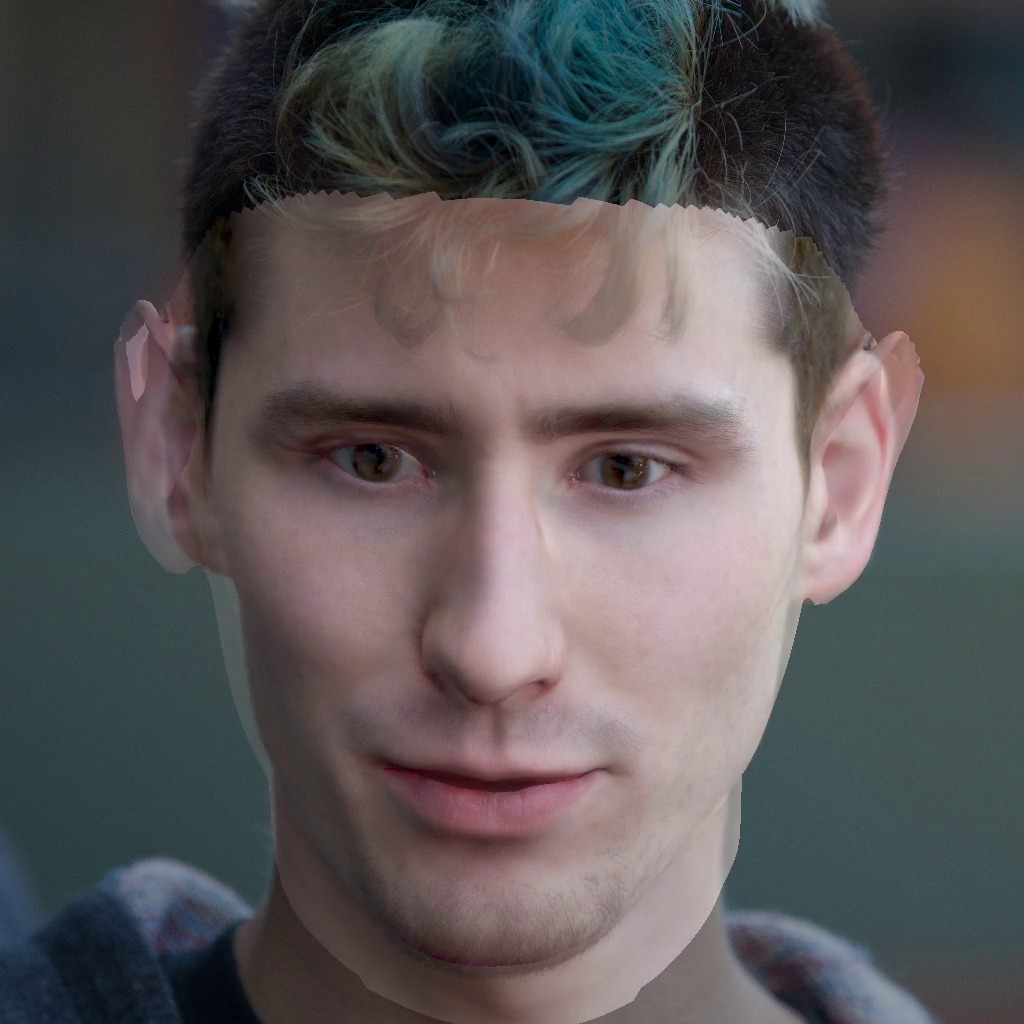
\includegraphics[width=0.8\textwidth]{figures/black-bg_no-aa}
    \caption{忽略可见性梯度,模型与照片未准确对齐}
    \label{fig:problem_a}
\end{subfigure}%
\begin{subfigure}[t]{0.5\textwidth}
    \centering
    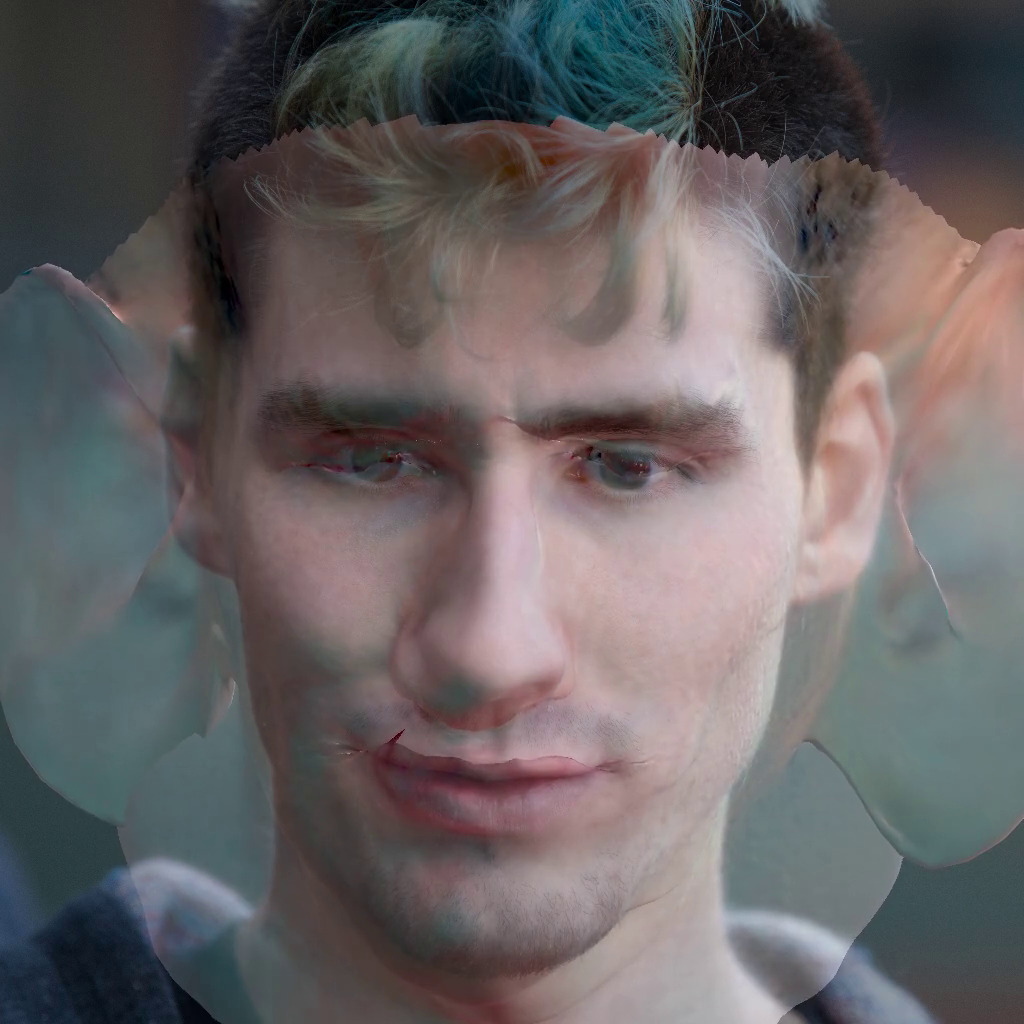
\includegraphics[width=0.8\textwidth]{figures/black-bg}
    \caption{使用全黑代替背景模型,可见性梯度错误}
    \label{fig:problem_b}
\end{subfigure}%
\caption[未知背景条件下可微分渲染优化结果]{
    未知背景条件下可微分渲染优化结果。
    示意图为渲染结果叠加在目标照片上。
}
\end{figure}

\begin{figure}
    \centering
    \import{build/figures/}{problem.pgf}
    \caption[在未知背景时计算可见性梯度困难]{
        在未知背景时计算可见性梯度困难。
        拟合目标(第一行)和渲染结果(第二行)左侧白色为前景,右侧为背景。
        在第二行中,前景模型为以红线为边界的白色平面。
        横坐标为前景模型的平移量。
        函数值为每像素均匀采样65536次的数值近似。
        (a)离散采样,不计算可见性梯度;
        (b)使用不准确的黑色背景模型计算可见性梯度,模型无法收敛到期望位置;
        (c)理想情况下,在完全已知背景时的可见性梯度,模型能准确收敛至梯度为0的点。
    }
    \label{fig:problem}
\end{figure}
本节将设计一个简单的玩具实验来更直观地说明上述问题。
如图\ref{fig:problem}所示,我们使用一个简单的白色平面作为前景模型,用其拟合一个白色青色对半分割的场景。
该模型的参数是其横向的平移量,用平面边缘与横坐标轴的交点$a_x$表示。
该平面的边缘稍微倾斜,以突出可见性梯度的变化。
该平面的着色不受参数影响,始终固定为白色。
该例子中使用的损失函数为L1误差,即:
\begin{equation}
\mathcal{L} = \left\| \hat{\mathcal{I}} - \mathcal{I} \right\|_1
\text{。}
\label{eq:loss_l1}
\end{equation}

在该实验中,如图\ref{fig:problem},(a)为离散采样的方式,也是目前大多人脸重建中使用的方法。
其渲染流程为:在每个像素的中点处采样,若其位于前景模型的覆盖范围内,则渲染为白色,否则渲染为背景色。
由于采样过程是离散的,且$a_x$的改变并不会影响采样的方式,因此,渲染结果$\hat{\mathcal{I}}$关于$a_x$的梯度为0,其损失函数为阶梯函数。
即该损失函数完全无法以基于梯度的方式指导模型拟合。

另一方面,在没有准确背景模型的前提下,可见性梯度则难以被利用。
例如,在(b)中,假设我们并不知道该场景的背景,因此直接假设其为全黑。
但在本例中这个假设显然是不准确的。
(b)和(c)的渲染方式与(a)不同,其每个像素的颜色取决于前景模型覆盖该像素的面积的比例,并按面积比例线性混合前景和背景的颜色。
这使得处于前景边缘处的像素的颜色成为了关于$a_x$的连续函数,即产生了所谓的可见性梯度。
在此前提下,从图中可以观察到其损失函数呈递减的趋势,并未在期望的位置上形成极值。
因此,该梯度也无法引导模型收敛到期望的位置。

作为参考,(c)展示了理想中,完全已知背景的情况下,可见性梯度的作用。
从图中可见,其损失函数在期望的位置上有一个明显的极值,且其周围的梯度将能很好地指导优化器,使模型收敛到该位置。

然而,在实际非受限环境照片的人脸重建的任务中,背景可能是很复杂且难以建模的。
本章将探讨在这种情况下,如何利用可见性梯度以指导前景模型与目标照片中的边缘对齐。

\subsection{现有人脸重建方法未利用可见性梯度}

现有的非受限环境人脸重建方法也都面临这个问题。
在使用了可微分渲染技术的方法中,它们均直接没有考虑人脸与背景间的可见性梯度。
为了在缺少这项梯度的情况下获得精确的人脸几何形状,他们通常会:
\begin{itemize}
\item 使用多目立体等其他手段事先确定高精度的人脸几何形状,并在逆渲染优化过程中使几何形状保持不变,仅在逆渲染过程中优化材质相关参数\citep{RiviereGBGB20}。
这限制了其可能的应用场景,这些方法必须使用多帧照片作为输入。
对人脸来说,拍摄多帧照片时人的姿态表情需要保持不变,这也提升了数据采集难度。
\item 使用2D人脸关键点提供监督信号\citep{deep3d}。
这种方案最大的问题是:部分关键点(例如脸颊上的)在人脸上的位置定义是不明确的,这导致监督信号中难免引入噪声。
虽然已有工作\citep{qu122015adaptive}通过“边缘关键点”的定义试图改善这种情况,但仍无法完全消除不明确的定义。
此外,在重建过程中引入人脸关键点检测模块也会增加算法的复杂度,并使重建精度受关键点检测精度的影响。
\end{itemize}
除人脸重建外,通用的3D重建研究也面临同样的问题,例如\citet{nvdiffrec}使用额外的图像分割结果作为监督。
但是,如果能够直接利用可见性梯度,可大大简化算法的流程,同时也能避免在前序步骤中引入额外的误差。

\subsection{现有考虑未知背景的方法适用范围有限}

\citet{SchonbornEFV15}讨论了在逆渲染的优化过程中对未知背景的处理。
但该方法是概率推理方法,其优化过程是不断在后验分布中采样,寻找最大似然的解。
该优化过程是离散的,其中并未使用到梯度,因此难以和神经网络等方法中基于梯度下降的优化方法相结合。
该作者提出的方法,例如每个像素假定有$p=0.8$的概率属于背景,也难以和常见的损失函数相结合。

而本章将提出一种新的损失函数,该函数能直接应用于图\ref{fig:inv_rendering}中损失函数的位置,
并能与现有各种有计算可见性梯度能力的可微分渲染方法结合,以梯度下降的方式监督任意模型的优化过程。

\section{面积归一化的像素损失函数}

本节将提出一种应用于可微分逆渲染的损失函数以解决上述问题。
为了结论的通用性和分析方便,本节将首先在连续(无限分辨率)的图像中定义该损失函数。
之后将其推广到使用离散的像素表示的图像中,并进一步分析其性质和与现有可微分渲染方法结合的实现方式。

在连续图像的分析中,不妨先将目标照片$\hat{\mathcal{I}}$和渲染结果$\mathcal{I}$抽象为连续的颜色场$\mathbb{R}^2 \to \mathbb{R}^3$,
即从二维像素坐标到RGB颜色值的映射。
于是公式\eqref{eq:loss_l1}中的原始L1损失函数可改写为:
\begin{equation}
\mathcal{L} = \iint_{\mathcal{A}} \left\| \hat{\mathcal{I}} - \mathcal{I} \right\|_1 \mathrm{d}\sigma +
\iint_{\mathcal{B}} \left\| \hat{\mathcal{I}} - \mathcal{I} \right\|_1 \mathrm{d}\sigma
\text{,}
\label{eq:loss_l1_area}
\end{equation}
其中,$\mathcal{A}$为渲染结果中前景模型覆盖的区域,$\mathcal{B}$为背景覆盖的区域,两者应互为补集。
由此我们可以对图\ref{fig:problem}b中的现象进一步地解释:
当前景模型的边界向右移动越过中点之后,由于不能很好地拟合背景,该损失函数的第一项开始上升,这是符合预期的。
但是,由于采用的背景模型不准确,背景部分也存在一定误差,且由于背景区域面积下降,损失函数的第二项将会下降。
这两项相互制衡,导致前景和背景模型“抢夺”处于交界处的像素。
若背景模型的误差足够大,以至于使用前景模型来拟合背景区域反而占优势,则会出现如图\ref{fig:problem}b中的现象:前景模型将在优化中不断抢占背景的区域,从而无法收敛到期望的位置。
在实际中这种情况是很有可能的,比如在3D人脸重建中,人脸的材质模型通常具有很高的自由度以拟合人脸的细节,这些自由度可能被误用于拟合背景。

为解决在未知背景下的逆渲染问题,本文提出了一种面积归一化的像素损失函数:
\begin{equation}
\mathcal{L}_n = \frac{\iint_{\mathcal{A}} \left\| \hat{\mathcal{I}} - \mathcal{I} \right\|_1 \mathrm{d}\sigma}
{\iint_{\mathcal{A}}\mathrm{d}\sigma}
-\alpha\iint_{\mathcal{A}}\mathrm{d}\sigma
\text{。}
\label{eq:loss_n}
\end{equation}
该损失函数仅在前景模型覆盖的区域内计算损失,因此不会受到背景模型的误差影响。
该函数第一项为单位前景区域面积内的平均误差,第二项鼓励更大的前景区域,$\alpha$为一个超参数。

\begin{figure}
\centering
\import{build/figures/}{one_dim_loss.pgf}
\caption{面积归一化的像素损失函数在一维的作用分析}
\label{fig:one_dim_loss}
\end{figure}

为了更好地理解该损失函数的作用,本文将展示一个一维情况下的简单例子。
如图\ref{fig:one_dim_loss}a所示,假设拟合目标包含前景和背景,为分段常函数;前景模型为定义在前景区域$\mathcal{A}=(0,\theta)$的常函数,$\theta$为模型参数:
\begin{align}
\mathcal{I}(x) &= \begin{cases}
    1   & x \leq 0.6 \\
    0.1 & x > 0.6
\end{cases}\\
\hat{\mathcal{I}}(x) &= 0.8 \quad x < \theta
\text{。}
\end{align}
在此定义下,我们可求出$\mathcal{L}_n(\theta)$中各项的解析表达式:
\begin{align}
\int_{\mathcal{A}} \left\| \hat{\mathcal{I}} - \mathcal{I} \right\|_1 \mathrm{d}\sigma
&= \int_0^{\theta} \left| \hat{\mathcal{I}}(x) - \mathcal{I}(x) \right| \mathrm{d}x \\
\int_{\mathcal{A}}\mathrm{d}\sigma &= \int_0^{\theta} \mathrm{d}x = \theta
\text{。}
\end{align}
其函数图像如图\ref{fig:one_dim_loss}b、c、d所示。
该函数第一项的分子为公式\eqref{eq:loss_l1_area}中的第一项前景部分,显然该项是随着$\theta$单调递增的。
由于没有了背景部分的制衡,单独使用该项将导致模型收敛到一个很小的区域。
于是本文将该项以前景区域的面积进行归一化,即$\mathcal{L}_n$的第一项。
若该模型的拟合误差在前景区域内是均匀分布的,则该项将会是一个常数,不会引导模型减小面积。
而模型拟合背景区域的误差通常显著大于拟合前景,因此该项鼓励模型离开背景区域,从而减小平均误差。
而在当前景区域小于目标时,$\mathcal{L}_n$的第二项将会鼓励模型增大面积,准确对齐到目标的边界上。如图\ref{fig:one_dim_loss}d所示,$\mathcal{L}_n$在$\theta=0.6$处取得极值,此时模型的前景区域正好对齐了目标的边界。
同时,若有拟合误差在前景边缘处大于中心的情况,第二项也能提供一定的补偿。
直观地,若拟合目标具有清晰的边界,且在边界处模型拟合前景的误差小于拟合背景的误差,则存在一个$\alpha$,使模型能精确对齐到该边界上。

上述例子推广到二维的情况会稍微复杂,因为在二维下边界不止一个点,而边界的不同位置将会有不同情况。但根据以上分析,本章提出的损失函数最适用于以下场景:
\begin{enumerate*}
    \item 背景复杂且未知,但拟合目标具有清晰的边界;
    \item 在前景物体边界附近的拟合误差不显著高于中心区域;
    \item 在边界上,模型拟合前景的误差小于拟合背景的误差。
\end{enumerate*}
若在边界的个别区段上不能满足上述条件,则需要通过一定的平滑等正则化方法进行补偿。
常见的情况比如:
由于景深浅,照片中物体边缘有较大模糊;
或者在部分位置碰巧前景与背景颜色相似等。

\section{收缩和扩展梯度分析}

本节将介绍如何将上一节提出的,定义在连续空间的损失函数应用于由离散的像素组成的图像上,
并分析了其梯度,提出了该损失函数更高效的等效实现。

为了使渲染图像$\hat{\mathcal{I}}$成为关于其渲染参数的的连续函数,本文将使用离散像素表示的图像渲染的过程定义为:
\begin{equation}
\hat{\mathcal{I}}(i;\theta) = (\mathbf{c}_i, \sigma_i)
\text{,}
\label{eq:rendering}
\end{equation}
其中$i$为像素索引,$\theta$为前景模型的渲染参数,
$\mathbf{c}_i\in\mathbb{R}^3$为着色后的像素颜色,且对前景模型覆盖区域外的像素没有定义,
$\sigma_i\in[0,1]$为前景模型覆盖该像素的覆盖率,即该像素中被模型覆盖的面积占其总面积的比例。
$\mathbf{c}$的值取决于所选择的着色模型,因此在本章中不考虑其关于$\theta$的梯度。
自然地,对于处在前景模型在图像上投影内部的像素$\sigma=1$,而对于模型外部的像素$\sigma=0$,
仅当像素位于模型边界上时,$\frac{\partial\sigma}{\partial\theta}$才不为0,因此处于模型边界上的覆盖率$\sigma$是本节主要考虑的对象。
需要注意的是,准确地求出每个像素的$\sigma$较为复杂,现有很多通用可微分渲染方法都在这方面做出了不小的努力。
后文第\ref{sec:method_discuss}节将基于现有通用可微分渲染方法,介绍一种基于nvdiffrast的高效实现方式。

基于该定义,我们可以将面积归一化的像素损失函数的定义推广至由离散的像素表示的图像中:
\begin{equation}
\mathcal{L}_n = \frac{\sum_{i} \sigma \left\| \mathbf{c} - \mathcal{I} \right\|_1}
{\sum_{i} \sigma} - \alpha \sum_{i} \sigma
\text{。}
\label{eq:loss_n_pixel}
\end{equation}
与之前定义在连续空间的公式\eqref{eq:loss_n}相比,该定义假设了同一个像素范围内的图像颜色保持不变。

下面将对该损失函数的梯度进行分析,以探寻其性质和可能的实现方式。
对公式\eqref{eq:loss_n_pixel}求导可得:
\begin{equation}
\frac{\partial\mathcal{L}_n}{\partial\theta} =
\sum_{i}\left[
    \frac{
        \overbrace{\textstyle \left\| \mathbf{c}_i - \mathcal{I}_i \right\|_1 \sum_j\sigma_j}^\text{收缩} -
        \overbrace{\textstyle \sum_j \sigma_j \left\| \mathbf{c}_j - \mathcal{I}_j \right\|_1}^\text{扩展}
    }{\left(\sum_j\sigma_j\right)^2} - \alpha
\right]\frac{\partial\sigma_i}{\partial\theta}
\text{。}
\label{eq:loss_n_pixel_gradient}
\end{equation}
注意在该推导中我们忽略了$\mathbf{c}$关于$\theta$的梯度,这项梯度由具体的着色模型确定,通常可以使用自动微分求得。
从该推导结果中可以发现以下特点:
\begin{enumerate*}
    \item 该梯度仅在$\frac{\partial\sigma}{\partial\theta}$不为0时才不为0,因此在计算时仅需考虑处于前景模型边界上的像素;
    \item 其大体可分为收缩和扩展两项,分别将鼓励模型向内收缩其边界和向外扩展其边界;
    \item 当模型边界进入背景区域时,收缩梯度由于边界处误差较大而较大,但扩展梯度由于只依赖于平均误差,因此上升幅度较小,此时收缩梯度将占主导地位,鼓励模型离开背景区域;
    \item 若拟合误差分布均匀,即$\left\|\mathbf{c} - \mathcal{I}\right\|_1$与像素坐标$i$或$j$无关,则收缩和扩展两项梯度相等,此时$\alpha$将轻微地鼓励扩展,以对齐边界。
\end{enumerate*}
这些特点均和之前的连续空间定义的损失函数相同。

虽然可以直接根据公式\eqref{eq:loss_n_pixel}使用自动微分计算梯度,
但其中的覆盖率$\sigma$仅在模型边界上才不为0,其余部分的$\sigma$并不需要保存到内存中。因此我们可以实现以下损失函数:
\begin{equation}
\tilde{\mathcal{L}}_n =
\underbrace{\frac{1}{|\mathcal{A}|}\sum_{i|\sigma\in(0,1)} \sigma\left\| \mathbf{c} - \mathcal{I} \right\|_1}_{\text{收缩}} -
\underbrace{\sg\left[\frac{\sum\sigma\left\| \mathbf{c} - \mathcal{I} \right\|_1}{|\mathcal{A}|^2}+\alpha\right]\sum_{i|\sigma\in(0,1)} \sigma}_{\text{扩展}}
\text{,}
\label{eq:loss_n_tilde}
\end{equation}
其中$|\mathcal{A}|$为优化开始时前景模型覆盖的面积,即$\sum_{i} \sigma$。
$\sg$为梯度停止操作符,表示在求导时该项视为常数。
依据该公式则仅需要处理位于前景模型边缘处的像素的覆盖率$\sigma$,其余部分则无需消耗额外的内存和计算资源。
注意此处列出的$\tilde{\mathcal{L}}_n$仅包含了模型与未知背景间的可见性相关梯度,在实际中需要配合通常的可微分渲染以计算颜色$\mathbf{c}$和其他已知背景的可见性梯度。

这个新定义的损失函数的梯度为:
\begin{equation}
\frac{\partial\tilde{\mathcal{L}}_n}{\partial\theta} =
\sum_{i}\left[
    \frac{
        \textstyle \left\| \mathbf{c}_i - \mathcal{I}_i \right\|_1 |\mathcal{A}| -
        \textstyle \sum_j \sigma_j \left\| \mathbf{c}_j - \mathcal{I}_j \right\|_1
    }{|\mathcal{A}|^2} - \alpha
\right]\frac{\partial\sigma_i}{\partial\theta}
\end{equation}
与之前的梯度结果\eqref{eq:loss_n_pixel_gradient}对比,该函数使用常数$|\mathcal{A}|$代替了变量$\sum_{i} \sigma$,以避免在每次迭代中计算前景模型覆盖面积。
由于基于梯度的逆渲染方法通常并不能处理大范围的模型移动,因此该项可以近似看作常数,不会带来太大的误差。
然而这样的替换会导致原本“面积归一化”部分带来的梯度缺失,
因此$\tilde{\mathcal{L}}_n$通过手动计算扩展项的系数补足了相关梯度。

根据以上分析,我们最终得到了一个附加的,仅定义在模型边缘处像素的损失函数。
该函数的目的是在逆渲染的优化中,产生额外的收缩与扩展两项梯度,从而促进模型对齐到与未知的背景的边缘。

\section{基于nvdiffrast的高效实现}

\begin{figure}[ht]
    \centering
    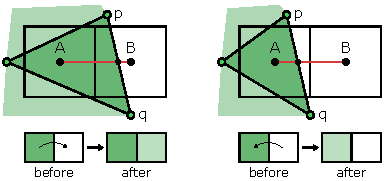
\includegraphics{figures/antialias}
    \caption[nvdiffrast抗锯齿模块的工作流程]{nvdiffrast抗锯齿模块的工作流程\citep{nvdiffrast}}
    \label{fig:aa}
\end{figure}
本文基于上文所述理论,基于nvdiffrast\citep{nvdiffrast}中的抗锯齿模块进行了实现。
该抗锯齿模块的作用为:对于每个处于模型相互遮挡的边缘的像素,该模块计算其覆盖率$\sigma$,并根据覆盖率调整该像素渲染颜色;对于其他不处于边缘的像素则不做处理。
如此一来,该模块虽然没有显式地输出覆盖率$\sigma$,但它使渲染结果成为了覆盖率的连续函数,该模块正是nvdiffrast中处理可见性梯度的关键。
然而,该模块工作时仍需要指定一个背景。
如图\ref{fig:aa}所示,该模块修改过的像素为左图的B和右图的A。
在该图的四个像素中,绿色的部分覆盖该像素的面积占整个像素面积的比例为覆盖率$\sigma$。
记修改前绿色部分的像素值为$\mathbf{c}$,白色背景的像素值为$\mathcal{J}$。
则修改后的像素值为:
\begin{equation}
\mathbf{c}' = \sigma\mathbf{c} + (1-\sigma)\mathcal{J}
\text{。}
\end{equation}

基于该模块,本文使用目标图像$\mathcal{I}$作为背景进行渲染,即$\mathcal{J}=\mathcal{I}$,则公式\eqref{eq:loss_n_tilde}中的收缩项可进一步表示为:
\begin{equation}
\sigma\left\| \mathbf{c} - \mathcal{I} \right\|_1 =
\left\| \sigma\mathbf{c} + (1-\sigma)\mathcal{I} - \mathcal{I} \right\|_1 =
\left\| \mathbf{c}' - \mathcal{I} \right\|_1
\text{,}
\label{eq:impl_nvdiffrast}
\end{equation}
其中$\mathbf{c}'$为在目标图像$\mathcal{I}$之上渲染前景模型而得到的渲染图像。如此便可将收缩项中的$\sigma$完全交给该抗锯齿模块处理。
更好的是,在同一抗锯齿模块中还可以同时处理其他已知背景部分的可见性梯度,例如下巴和脖子间,鼻子和脸颊间。

但nvdiffrast的覆盖率计算是稀疏的,即有部分$\sigma\in(0,1)$的像素无法被检测到,检测的概率和所用3D模型的网格密度有关。
而扩展项的梯度与收缩项相互制衡,因此其梯度的计算必须与收缩项相互耦合,即他们稀疏的模式必须相同。
又注意到扩展项的梯度的大小对于边缘的每一个像素是均匀的,%因此本实现直接在反向传播时,对所有实际检测到$\sigma\in(0,1)$的像素添加上该项梯度。该方法也基本无额外内存和运算开销。
因此本文在实现扩展项梯度时,直接修改了nvdiffrast的CUDA代码,
在前向传播的过程中,本文利用其位域中尚未使用的空间,标记了所有前景模型和未知背景间所有实际检测到的边缘像素对,
并额外输出一个占位变量$\tilde{\sigma}$,该变量的值没有定义,它仅用于接收PyTorch自动求导框架传递的扩展项梯度的系数,以此避免在每次前向传播中计算前景模型覆盖的总面积。
在反向传播的过程中,本文直接将占位变量获得的梯度,传递到所有之前标记的边缘上,从而实现了扩展项梯度的计算。
在计算损失函数\eqref{eq:loss_n_tilde}时,$\tilde{\sigma}$将取代$\sum\sigma$用于从PyTorch中接收扩展项梯度。

基于以上介绍的收缩和扩展项的实现方式,在基于nvidffrast的实现中,最终可在PyTorch的代码中编写的损失函数为:
\begin{equation}
\tilde{\mathcal{L}}_n = \frac{1}{|\mathcal{A}|} \sum \left\| \mathbf{c}' - \mathcal{I} \right\|_1 - e \tilde{\sigma},
\quad e = \frac{\sum\left\| \mathbf{c}' - \mathcal{I} \right\|_1}{|\mathcal{A}|^2}+\alpha
\label{eq:loss_n_impl}
\end{equation}
其中$e$为扩展项的梯度的系数。由于$\tilde{\sigma}$的值没有定义,因此在梯度时应将$e$视为常数(在PyTorch中调用\texttt{detach()}),防止向它传递错误的梯度。
基于该实现的整个逆渲染流程如算法\ref{alg:impl_nvdiffrast}所示。
\begin{algorithm}[t]
    \caption{基于nvdiffrast的逆渲染流程}
    \label{alg:impl_nvdiffrast}
    \begin{algorithmic}[1]
        \Require 前景渲染模型$\hat{\mathcal{I}}$,模型参数初始化$\theta^{(0)}$,目标图像$\mathcal{I}$
        \Procedure{逆渲染优化}{$\theta^{(0)}$, $\mathcal{I}$}
            \State 计算前景区域面积$|\mathcal{A}|$
            \For{$i=1$ to $N$}
                \State $\mathbf{c} \gets \hat{\mathcal{I}}\left(\theta^{(i-1)}\right)$
                    \Comment{前景模型逐像素正向渲染}
                \State $\mathbf{c}_j \gets \begin{cases} \mathbf{c}_j &\text{if } j\in\mathcal{A} \\ \mathcal{I}_j &\text{otherwise} \end{cases}$
                    \Comment{将前景渲染于目标图像之上}
                \State $\mathbf{c}', \tilde{\sigma} \gets \text{抗锯齿模块}(\mathbf{c})$
                \State $\tilde{\mathcal{L}}_n \gets \frac{1}{|\mathcal{A}|} \sum \left\| \mathbf{c}' - \mathcal{I} \right\|_1 - e \tilde{\sigma}$
                    \Comment{计算损失函数,公式\eqref{eq:loss_n_impl}}
                \State $\theta^{(i)} \gets \theta^{(i-1)} - \eta \nabla_{\theta} \tilde{\mathcal{L}}_n$
                    \Comment{利用PyTorch的自动微分计算梯度并更新参数}
            \EndFor
            \State \Return $\theta^{(N)}$
        \EndProcedure
    \end{algorithmic}
\end{algorithm}

nvdiffrast的稀疏覆盖率检测有时会导致整体梯度估计的偏差过大,进而导致模型不能收敛到期望的位置,
因此可能还需要手动将相关梯度乘以一个放大系数进行补偿。
下文将对该问题进一步讨论,并提出另一种缓解措施。

\subsection{性能分析}

nvdiffrast的特点正是以渲染和反向传播性能较高。
而本章所提出的基于它的实现也继承了这一特点,本章在nvdiffrast之上几乎没有增加额外的性能开销。
本文通过将前景模型渲染于目标图像之上的方式实现收缩项梯度,其运行时开销和正常渲染相同。
而扩展项所使用的标记利用了现有位域中的空间,因此不会增加额外的内存开销。
在计算量上,除了在优化开始前需要计算一次前景模型的覆盖面积$|\mathcal{A}|$外,
其余每次迭代每张图片所需的额外计算仅有扩展项梯度的系数$e$,以及边缘像素的一次额外梯度累加。
这些计算相比于模型渲染过程来说可以忽略不计。

\section{实验结果}

\subsection{立方体姿态估计}

与SoftRas\citep{softras}类似,本文设计了一个仅使用可微分渲染估计立方体姿态的实验。
该实验将一个确定的,但每个面具有不同颜色的立方体放置在场景中的随机位置,并使用随机且未知的背景渲染一张图像。
然后使用本章所述的方法对该图像进行逆渲染,以恢复立方体的姿态。
在该实验中,立方体每个面均是纯色,因此着色的步骤将不会产生梯度。
该优化过程中所利用的梯度仅来自于不同面之间,立方体与背景间的可见性梯度。

\paragraph{实现细节}
生成随机背景时,背景四个角的颜色从立方体六个面使用的六种颜色中随机选择,
其余部分的颜色则从该四个角的颜色中双线性插值得到。
如SoftRas中所述,该优化问题有很多局部最优点,但本文的重点并不在此。
因此本文选择在立方体姿态真实值附近随机生成初始值,以提高优化的成功率。
具体方法为,立方体的棱长为$2$,立方体中心坐标均匀分布在真值附近的$[-0.3,0.3]^3$的立方体内,
并绕任意旋转轴关于其中心旋转$[0,15°]$的角度。
该优化过程使用上述基于PyTorch\citep{pytorch}和nvdiffrast实现,被优化的参数是表示SE(3)变换的6个参数。
优化的目标函数为公式\eqref{eq:loss_n_impl},且未使用任何正则项。
本文使用Adam\citep{adam}优化器,学习率为$2\times 10^{-4}$,其余参数为默认值。
渲染的分辨率为$128\times128$,运行了4000次优化迭代。
本实现在NVIDIA RTX3060显卡上,在批大小128的情况下,每秒能运行约180次优化迭代,整个优化过程需要约27秒。
为保证公平对比,以下实验结果中,每种方法均对相同的2048张随机图像进行了测试,每种方法优化的初始化位置也是相同的。

\begin{table}
    \centering
    \caption{立方体逆渲染的实验结果}
    \label{tab:cube_opt}
    \begin{tabular}{l|rrr}
        \toprule
        方法       & 成功率(\%) & 旋转误差(°) & 位置误差 \\
        \midrule
        初始化      &  6.15 & 3.71 & 0.294 \\
        黑色背景    & 67.14 & 1.53 & 0.234 \\
        数学期望背景& 91.02 & 0.59 & 0.064 \\
        本文方法    & \textbf{96.19} & \textbf{0.40} & \textbf{0.035} \\
        \midrule
        理想背景    & 98.83 & 0.06 & 0.001 \\
        \bottomrule
    \end{tabular}
\end{table}
表\ref{tab:cube_opt}展示了不同背景模型下优化的成功率与收敛精度的对比。
其中,优化后的最终姿态与真实姿态间旋转误差小于$5°$视为优化成功,后续的旋转误差与位置误差均只在成功的例子中计算。
可见不论使用何种背景模型,使用可见性梯度均能有效引导模型优化。
但使用更准确的模型将能得到更好的优化结果。
例如,相比于使用黑色背景,通过引入少量关于背景随机生成的先验知识,使用随机过程的数学期望作为背景能显著够提高优化的成功率。
然而,在非受限环境照片的人脸重建任务中,这样的先验可能难以获得。
相比之下,本文的方法在无需任何先验的情况下,仍有更高的成功率,且在成功的例子中,收敛的精度也显著更高,其误差在前述基线方法的一半以下。
但若以每张目标图片生成时使用的准确背景作为背景模型,则能获得远高于以上未知背景的结果。

\begin{figure}
    \centering
    \begin{tikzpicture}[
        node distance=2pt and 0pt,
        image/.style={inner sep=0pt, outer sep=0pt},
    ]
        \node (a) [image] {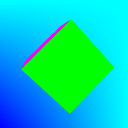
\includegraphics[width=1.05in]{figures/cube_opt/target/110.png}};
        \node (b) [image,right=of a] {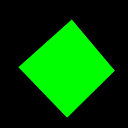
\includegraphics[width=1.05in]{figures/cube_opt/init/110.png}};
        \node (c) [image,right=of b] {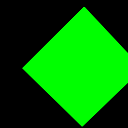
\includegraphics[width=1.05in]{figures/cube_opt/black/110.png}};
        \node (d) [image,right=of c] {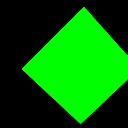
\includegraphics[width=1.05in]{figures/cube_opt/exp/110.png}};
        \node (e) [image,right=of d] {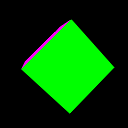
\includegraphics[width=1.05in]{figures/cube_opt/my/110.png}};
        \node (f) [image,right=of e] {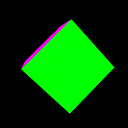
\includegraphics[width=1.05in]{figures/cube_opt/truth/110.png}};

        \node (a) [image,below=of a] {
\includegraphics[width=1.05in]{figures/cube_opt/target/49.png}};
        \node (b) [image,right=of a] {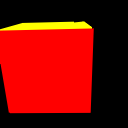
\includegraphics[width=1.05in]{figures/cube_opt/init/49.png}};
        \node (c) [image,right=of b] {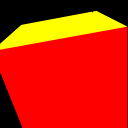
\includegraphics[width=1.05in]{figures/cube_opt/black/49.png}};
        \node (d) [image,right=of c] {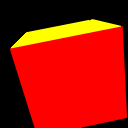
\includegraphics[width=1.05in]{figures/cube_opt/exp/49.png}};
        \node (e) [image,right=of d] {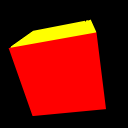
\includegraphics[width=1.05in]{figures/cube_opt/my/49.png}};
        \node (f) [image,right=of e] {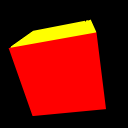
\includegraphics[width=1.05in]{figures/cube_opt/truth/49.png}};

        \small
        \node [below=of a] {(a)目标图像};
        \node [below=of b] {(b)初始化};
        \node [below=of c] {(c)黑色背景};
        \node [below=of d] {(d)数学期望背景};
        \node [below=of e] {(e)本文方法};
        \node [below=of f] {(f)理想背景};
    \end{tikzpicture}
    \caption[立方体的位置和姿态的收敛情况可视化]{
        立方体的位置和姿态的收敛情况可视化。
        (a)立方体渲染于随机背景上的优化目标图像;
        (b)优化前初始化的立方体姿态;
        (c)使用黑色背景模型的优化结果;
        (d)使用随机背景的数学期望作为背景模型的优化结果;
        (e)使用本文方法的优化结果;
        (f)直接使用渲染目标图像时使用的背景的优化结果。
    }
    \label{fig:cube_opt_vis}
\end{figure}
图\ref{fig:cube_opt_vis}可视化了两组实验的结果。
可见若使用不准确的的黑色或数学期望背景模型,则优化过程很容易受到背景中与前景相似的颜色的影响,导致无法正确收敛。
(c)、(d)、(e)对比可以看出越准确的背景模型可产生越好的优化结果。
不准确的背景模型会导致优化过程使用前景模型拟合背景,从而过度扩大前景的覆盖范围。
这证实了在一般的可微分渲染应用中,准确的背景模型的必要性。
而利用本章提出的方法即可在不对背景进行建模的情况下,以较高的概率得到准确的结果。

但在该实验中仍有少量的例子无法正确收敛,经可视化分析,这些例子可能依然在优化中陷入了局部最优。
为了进一步直接验证本章所提出的面积归一化的像素损失是否确实能在期望的位置上产生极值点,
本文开展了另一组实验。
在上述设置的基础上,该组实验将立方体旋转初始化范围减小到$1°$内,位移范围减小到$0.05$,且优化迭代次数降低为2000次,在如此小的范围内可完全排除局部最优的影响。

\begin{table}
    \centering
    \caption{立方体逆渲染的极值点测试结果}
    \label{tab:cube_opt2}
    \begin{tabular}{l|rrr}
        \toprule
        方法       & 成功率(\%) & 旋转误差(°) & 位置误差 \\
        \midrule
        初始化      & 100.00 & 0.70 & 0.048 \\
        黑色背景    & 86.91 & 1.19 & 0.143 \\
        数学期望背景& 97.12 & 0.46 & 0.041 \\
        本文方法    & \textbf{100.00} & \textbf{0.02} & \textbf{0.001} \\
        \bottomrule
    \end{tabular}
\end{table}
这组实验的结果如表\ref{tab:cube_opt2}所示。
可见本章提出的损失函数确实能在未知背景的情况下正确产生极值点。
本章方法不仅在所有例子中均能正确收敛,且收敛的精度高于对比的基线方法一个数量级以上。
相比之下,如果使用非常不准确的黑色背景,其结果甚至比初始化时更低。
\begin{figure}
    \import{build/figures/}{loss_vs_rot.pgf}
    \caption{损失函数与旋转误差的关系}
    \label{fig:loss_vs_rot}
\end{figure}
如图\ref{fig:loss_vs_rot}展示了在迭代优化过程中不同方法的损失函数和旋转误差的变化情况。
图中数据为128张随机图像的平均值。
从图中可见虽然每种方法的损失函数都在优化中不断下降,
但如果使用不准确的背景模型,旋转误差却反而会上升。
这证明了本章提出的损失函数可以在误差的零点处正确产生极值点,而使用不准确的背景模型则不能。

\subsection{3D人脸重建}

\TODO{与无法正常收敛的、不使用可见性梯度的、使用关键点监督的对比,展示没有SDF的局限性}

然而,该方法直接应用到人脸时会受到人脸模型人工裁剪的边缘的影响而无法获得理想的效果。
第\ref{chap:recon}章中将介绍本文如何解决该问题,并介绍将本章方法应用到人脸重建的更多实验。

\section{讨论}
\label{sec:method_discuss}

\paragraph{L1距离的必要性}
本文中所有的讨论都是基于渲染图像与目标图像的L1距离的,之所以不使用L2或其他距离,主要是基于以下原因:
\begin{itemize}
\item 直接的原因是公式\eqref{eq:impl_nvdiffrast}中$\sigma$和求距离的运算的交换需要L1距离。
\item 根本的原因是若将图像看作二维连续函数的离散化,则离散化的操作应尽可能小地对优化造成影响。
使用L1距离才能实现与像素离散化的方式无关的可见性梯度。
如图\ref{fig:problem}c所示,虽然该例子中图像分辨率很低,但其损失函数的梯度仍然是非常平滑的,并未受到像素离散化的影响。
图\ref{fig:l2_loss}展示了另一个使用L2损失的玩具实验的效果。
可见其梯度在像素边缘处出现了明显的阶跃,这是由像素离散化造成的。甚至在像素边缘处得到了为0的梯度,这显然是不合理且不利于优化的。
\end{itemize}

\begin{figure}
    \centering
    \import{build/figures/}{l2_loss.pgf}
    \caption[L2损失与像素离散化相关]{L2损失与像素离散化相关,各图含义参见图\ref{fig:problem}。}
    \label{fig:l2_loss}
\end{figure}

\paragraph{nvdiffrast可见性梯度稀疏的缓解}
前文提到,nvdiffrast的抗锯齿模块计算的覆盖率是稀疏的,即它会错过部分$\sigma\in(0,1)$的像素。
该问题的原因在于其检测渲染图像中不连续性(即包含前景和背景相互遮挡)的方式。
该模块判定相邻两个像素不连续当且仅当:
\begin{enumerate*}
\item 两个像素渲染自不同的三角形;
\item 其中来自前景的(深度较浅的)三角形在相机视角中处于物体边缘。
\end{enumerate*}
其中,处于边缘的判定方法为:来自前景的三角形满足以下条件之一:
\begin{enumerate*}
\item 在背景方向上无与其相邻的三角形;
\item 在背景方向上与其相邻的三角形朝向相机背面。
\end{enumerate*}
然而,真正处于边缘的三角形可能并未被渲染图像的任何一个像素采样到。
处于边缘的三角形被采样到的概率正比于其在渲染图像上的投影面积。
但为了提升精度而使用更高密度的网格会导致每个三角形面积的下降;
更雪上加霜的是,位于边缘的三角形的法向通常与相机方向夹角很大,导致其在渲染图像上的投影面积更小。
最终导致即使使用很高的分辨率也无法实现令人满意的采样概率。

为缓解该问题,本文提出放松处于边缘的判定条件,添加一条:背景未被任何三角形覆盖。
在该条件下即可保证与未知背景交界的所有边缘均被检测到。
但付出的代价是部分梯度不能正确地传递到真正处于边缘的顶点上,
而是被传递到与边缘相近的被采样到的三角形的顶点上。
但是在完整的优化问题中通常都具有鼓励模型局部光滑的正则项,这些梯度的影响最终将被较为均匀地分布到更大的区域上,因此这些偏差应该不会造成太大的影响。
图\ref{fig:vis_grad}展示了一些具体的例子。

此外,该方法只能缓解模型与未知背景间的不连续性判定,而对模型自身不同部分的遮挡无能为力。
这会导致内部的可见性梯度偏小,从而导致整体梯度估计发生偏差。
其具体影响需根据实际应用进一步分析。

\begin{figure}
    \centering
    \begin{subfigure}{0.33\textwidth}
        \centering
        \begin{tikzpicture}
            \path[use as bounding box] (-0.5,-0.5) rectangle (4,2.5);
            \draw [help lines] (0,0) grid [step=2cm] (4,2);
            \draw[red, name path=H] (1,1) -- (3,1);
            \filldraw (1,1) circle (1pt) node [above] {A}
                      (3,1) circle (1pt) node [above] {B};

            \coordinate [label=right:p] (p) at (1.2,2.2);
            \coordinate [label=right:q] (q) at (2,-0.3);
            \coordinate (r) at (-0.5,1);

            \draw (p) -- (r) -- (q);
            \draw [green!30!black, name path=T, thick] (p) -- (q);
            \path [name intersections={of=H and T,by=I}];

            \draw[fill=green] (p) circle (2pt);
            \draw[fill=green] (q) circle (2pt);
            \draw[fill] (I) circle (1pt);

            \begin{pgfonlayer}{background}
                \fill[green!50] (p) -- (1.1, 2.5) -- (-0.5,2.5) -- (-0.5,-0.3) --  (-0.5,-0.5) -- (2, -0.5) -- (q);
                \fill[green!80!black] (p) -- (q) -- (r) -- cycle;
            \end{pgfonlayer}
        \end{tikzpicture}
        \caption{正常检测到的边缘}
    \end{subfigure}%
    \begin{subfigure}{0.33\textwidth}
        \centering
        \begin{tikzpicture}
            \path[use as bounding box] (-0.5,-0.5) rectangle (4,2.5);
            \draw [help lines] (0,0) grid [step=2cm] (4,2);
            \draw[red, name path=H] (1,1) -- (3,1);
            \filldraw (1,1) circle (1pt) node [above] {A}
                      (3,1) circle (1pt) node [above] {B};

            \coordinate [label=above:p] (p) at (1.2,2.2);
            \coordinate [label=below:q] (q) at (2,-0.3);
            \coordinate (r) at (-0.5,1);
            \coordinate (s) at (2.2,2.2);
            \coordinate (t) at (2.6,-0.3);

            \draw (p) -- (r) -- (q);
            \draw (s) -- (t) -- (q) -- cycle;
            \draw (s) -- (p);
            \draw [green!30!black, name path=T, thick] (p) -- (q);
            \path [name intersections={of=H and T,by=I}];

            \draw[fill=red] (p) circle (2pt);
            \draw[fill=red] (q) circle (2pt);
            \draw[fill=gray!50] (s) circle (2pt);
            \draw[fill=gray!50] (t) circle (2pt);
            \draw[fill] (I) circle (1pt);

            \begin{pgfonlayer}{background}
                \fill[green!50] (s) -- (2.1, 2.5) -- (-0.5,2.5) -- (-0.5,-0.3) --  (-0.5,-0.5) -- (2.6, -0.5) -- (t);
                \fill[green!80!black] (p) -- (q) -- (r) -- cycle;
            \end{pgfonlayer}
        \end{tikzpicture}
        \caption{缓解情况1}
    \end{subfigure}%
    \begin{subfigure}{0.33\textwidth}
        \centering
        \begin{tikzpicture}
            \path[use as bounding box] (-0.5,-0.5) rectangle (4,2.5);
            \draw [help lines] (0,0) grid [step=2cm] (4,2);
            \draw[red, name path=H] (1,1) -- (3,1);
            \filldraw (1,1) circle (1pt) node [above] {A}
                      (3,1) circle (1pt) node [above] {B};

            \coordinate [label=above:p] (p) at (0.6,2.2);
            \coordinate [label=right:q] (q) at (2.2,-0.3);
            \coordinate (r) at (0.5,-0.2);
            \coordinate (s) at (2.2,2.2);

            \draw (p) -- (r) -- (q);
            \draw (q) -- (s) -- (p);
            \draw [green!30!black, name path=T, thick] (p) -- (q);
            \path [name intersections={of=H and T,by=I}];

            \draw[fill=red] (p) circle (2pt);
            \draw[fill=green] (q) circle (2pt);
            \draw[fill=gray!50] (s) circle (2pt);
            \draw[fill] (I) circle (1pt);

            \begin{pgfonlayer}{background}
                \fill[green!50] (s) -- (2.1, 2.5) -- (-0.5,2.5) -- (-0.5,-0.3) --  (-0.5,-0.5) -- (2.2, -0.5) -- (q);
                \fill[green!80!black] (p) -- (q) -- (r) -- cycle;
            \end{pgfonlayer}
        \end{tikzpicture}
        \caption{缓解情况2}
    \end{subfigure}
    \caption[nvdiffrast可见性梯度稀疏的原因及其缓解方法]{nvdiffrast可见性梯度稀疏的原因及其缓解方法。
    (a)展示了可正常检测到可见性梯度的情况,即A像素的采样点正好落在处于边缘的三角形上。其中绿色顶点表示梯度正确传递的顶点。
    (b)、(c)展示了两种常见的检测失败的情况,灰色顶点表示本应获得可见性梯度却未获得的顶点。
    (b)情况常见于脸颊与背景间,相机视线与表面法线夹角大,每个三角形的投影面积被大幅压缩,导致被采样到的概率减小。
    (c)情况常见于模型被裁剪的边缘,部分三角形与模型边缘仅有一个点连接,这些三角形有较高概率被A像素采样,却不被识别为处于边缘。
    本文提出的方法能在B像素采样到背景时,通过将本应传给灰色顶点的可见性梯度转而传递给红色像素,从而缓解该问题。}
    \label{fig:vis_grad}
\end{figure}

\paragraph{局限性}

虽然本章提出的方法能在一定程度上解决在未知背景时的逆渲染问题,但该方法仍然不如直接采集真实的背景图像,并对整张图片应用常规可微分渲染方法好。
本章方法中的超参数$\alpha$的选择与模型拟合误差的分布有关,如果拟合误差在空间上分布非常不均匀,或前景与背景差别过小则可能无法找到合适的参数。
此外,失焦造成的边缘模糊,以及碰巧背景颜色与人脸较为相近的情况下,本算法的对齐质量也会下降。

因此,如采用三脚架等固定机位拍摄时,则应该尽量在拍摄的同时采集真实背景,即保持相机位置和拍摄参数不变,分别拍摄有人在画面中的和仅有背景的照片。

\section{未来工作}

本章方法充分利用了人脸模型和背景间的可见性梯度,但从另一个方面说,也依赖这些梯度的正确性。
例如,当照片中的人物佩戴眼镜或其他饰品,导致照片中的人脸部分大幅偏离人脸模型的预测时,
本章方法将试图错误地将被饰品遮挡的部分移动到背景,从而导致错误的重建结果。
因此,未来的研究方向之一是如何将本章方法与异常数据检测方法结合,以排除这些干扰,提升算法的鲁棒性。
与神经网络相结合也是抵御数据噪声的一种可行方法。

本章在3D人脸重建的背景下提出了面积归一化的像素损失函数,但该损失函数的设计并不特定于人脸重建,也可以用于各种其他使用到可微分渲染的场景中。
该方法特别适合于满足如下条件的场景中:
\begin{itemize}
    \item 数据采集场景多样,因而照片中的背景难以建模或捕获;
    \item 前景部分有较为明确的先验模型,如在人脸中应用的的3DMM。
\end{itemize}
即先验信息集中于前景,而缺乏关于背景的先验信息的场景。
例如可应用于跟踪视频中出现的物体等。
该方法在多视角或多帧视频输入的重建中的应用也还有待探索。
更多的信息可能使得本方法更加鲁棒;但多帧图像之间的匹配信息原本即可用于重建3D模型,这可能导致本方法的必要性降低。

本章所介绍的损失函数在实现上并不简单,本章介绍了一种基于nvdiffrast的实现方式。
但从理论上来说,本章的方法也应能适用于其他考虑了可见性梯度的可微分渲染方法中。
例如基于redner\citep{redner}的光线追踪渲染时,可将收缩和扩展梯度集成于其边缘采样的过程中,正如与nvidiffrast中的抗锯齿模块的集成一样;
基于NeRF\citep{nerf}的体渲染方案则可将积分后的密度处于某一范围内的部分视为边缘,并应用收缩和扩展梯度。
这方面还有待进一步的研究。

\section*{本章小结}

本章提出了一种可适应未知背景的可微分逆渲染方法,该方法能够在无需对背景建模的境况下,将前景模型(如人脸)拟合到目标图像中。
本章首先将图像视为连续函数,提出了一种面积归一化的像素损失函数,
并在一维情况下对其进行了分析,说明了其可以有效帮助模型对齐到期望的边缘。
随后本章将损失函数推广到离散到像素的图像上,并进一步分析了其梯度,将梯度分为收缩和扩展两项,说明了推广后的损失函数的作用机理。
在此基础上,利用了其梯度仅在模型与背景交界处不为0的特点,本章提出了一种更高效的实现方式:在nvdiffrast的抗锯齿模块的基础上,在几乎不增加额外计算和存储开销的情况下实现了本章所述方法。
最后通过实验验证了本章提出的方法确实能实现在未知背景下的逆渲染,
并进一步讨论了本章方法可能的改进方向和在其他方面可能的应用。
第\ref{chap:recon}章将进一步介绍本章方法在人脸重建中的实际应用。
